\documentclass[presentation]{beamer}
\usepackage{../oop-slides-casadei}
\setbeamertemplate{bibliography item}[text]
\newcommand{\lessonnr}[0]{10}
\title[OOP10 -- DVCS Workflow and Lambdas]{10\\ Workflow per DVCS \\ Lambda expression e Stream}

\begin{document}

\frame[label=coverpage]{\titlepage}

%====================
%Outline
%====================
\begin{frame}<beamer>
 	\frametitle{Outline}
 	\tableofcontents[]
\end{frame}



\section{DVCS Workflow}

\subsection{Introduzione}

\fr{Dalle puntate precedenti} {
	\bl{DVCS} {
		\iz {
			\item DVCS sono strumenti potenti per tenere traccia in maniera efficiente della storia di un progetto
			\item Nascono in particolare come evoluzione dei tradizionali VCS (SVN, CVS \dots) 
			\item Enfasi su una \textbf{miglior gestione del lavoro di team}
		}
	}
	\bl{DVCS e teamwork} {
		\iz {
			\item ``La potenza \`e nulla senza controllo!'' 
			\item Ovvero \dots la mancanza di un metodo chiaro e condiviso per utilizzarli può portare a risultati \textbf{DEVASTANTI} 
            \iz {
                \item effort necessario per la parte di gestione diventa presto preponderante e insostenibile            
            }
			\item Ecco perch\'e nella pratica quotidiana, \`e bene adottare un \textbf{workflow collaborativo}
            \iz {
                \item i vostri progetti e i vostri partner di progetto vi ringrazieranno!            
            }
		}
    }
}

\fr{DVCS Workflow} {
	\bl{Cos'è} {
        \iz {
			\item E' una sorta di ``protocollo'', un insieme di regole e passi da seguire quando si utilizza un DVCS
			\item Essendo \textbf{collaborativo} by definition, ciascun team member vi partecipa con un \textbf{ruolo}
			\item Associa le diverse fasi del ciclo di vita del software a una serie di attività
            \iz {
                \item Ogni ruolo la/le proprie attività, ognuna codificata in un insieme di passi da seguire         
            }
		}
		
	}
	\bl{Come deve essere} {
		\iz {
			\item In tre aggettivi
            \iz {
                \item Semplice
                \item Chiaro
                \item Condiviso          
            }
		}
    }
}

\subsection{Caratteristiche di un workflow}

\fr{L'importanza dei ruoli} {
        \iz {
			\item Occupandosi di team collaboration, è naturale che il workflow definisca dei ruoli
			\item Nei progetti del ``mondo reale'' il set minimo di ruoli è composto da:
            \iz{
                \item i \textbf{developer}: sviluppano codice, implementano nuove funzionalità, bugfixing di funzionalità già rilasciate

                \item il \textbf{team leader}: coordina l'attività dei developer, sviluppa egli stesso (spesso si prende carico degli aspetti più delicati)

                \item il \textbf{release manager}: si occupa di gestire i rilasci, ovvero ``pubblicazione'' agli utenti delle nuove funzionalità del software
            }
		}	
}

\fr{Le attività coperte} {
        \iz {
			\item Sono quelle tipiche del cosiddetto \emph{software lifecycle}
            \iz{
                \item Sviluppo di nuove funzionalità

                \item Rilascio delle nuove funzionalità (dopo opportuni test funzionali)

                \item Fix di bug riscontrati nelle versioni rilasciate (tipicamente a seguito di segnalazioni da parte degli utenti)
            }
            \item Versioni? Cioè?
		}	
}

\fr{Le versioni} {
        \iz {
			\item Ogni rilascio del software è caratterizzato da una versione, identificata da un \textbf{numero}
            \item il numero ha (o dovrebbe) avere un senso, non è un numero estratto a sorte!
            \item Il pattern tipico è: \textbf{X.Y.Z} (numeri naturali)
            \iz{
                \item \textbf{X - major version}. Identifica una evoluzione importante di un software, nella quale funzionalità precedenti possono in generale aver subito modifiche o essere state eliminate.
                    \iz{
                        \item Retrocompatibilità non garantita!                    
                    } 
                \item \textbf{Y - minor version}. Identifica rilasci che aggiungono nuove funzionalità, senza toccare quelle già presenti. 
                    \iz{
                        \item Retrocompatibilità garantita!                    
                    } 
                \item \textbf{Z - bugfix version}. Identifica la risoluzione di difetti su una certa release \emph{X.Y}, senza aggiunta, modifica e/o cancellazione di funzionalità
                    \iz{
                        \item Retrocompatibilità garantita!                    
                    } 
            }
            \item Un buon riferimento è: \url{http://semver-ftw.org/}
		}	
}

\fr{Quale workflow} {
        \iz {
			\item Come si sceglie un workflow?
            \item Abbiamo parlato di semplicità...
            \item In realtà è più corretto parlare di giusto \textbf{trade-off} tra semplicità ed esigenze
		}	
}

\subsection{Due esempi di workflow}

\fr{Lo stato dell'arte I} {
%Definito da \emph{Vincent Driessen} e spiegato in \url{http://nvie.com/posts/a-successful-git-branching-model/}
\begin{center}
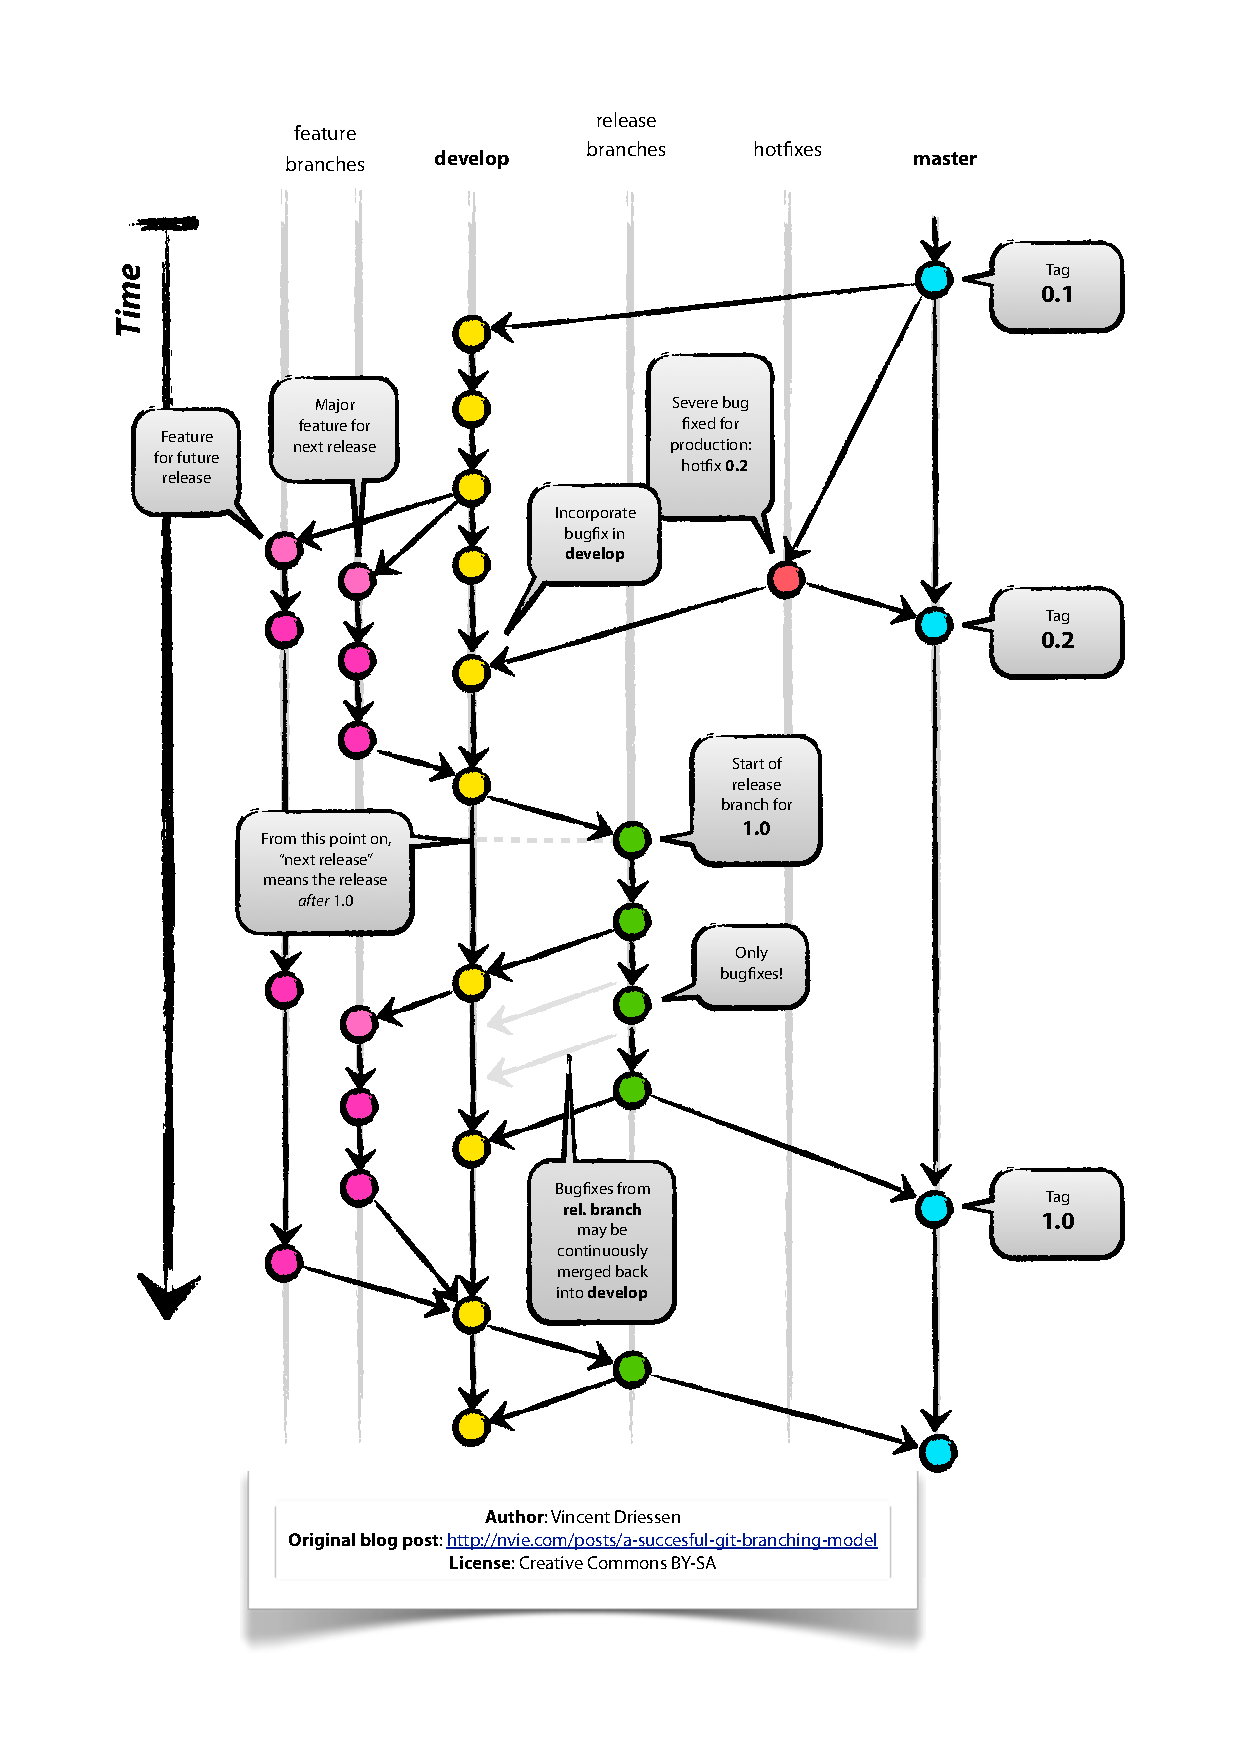
\includegraphics[width=0.5\textwidth]{img/Git-branching-model}
\end{center}
}

\fr{Lo stato dell'arte II} {
    \bl{Alcune considerazioni} {    
        \iz {
            \item Pensato per GIT (ma adottabile anche su Mercurial)
			\item Non lo useremo
            \iz{
                \item troppo complicato per i nostri scopi            
            }
            \item Comunque molto interessante perché racchiude tutti gli aspetti di un DVCS workflow
        }
    }

    \bl{Le branch} {
		\iz {
			\item Sono il supporto fondamentale alle fasi del ciclo di vita del software 
			\item Ogni fase la propria branch! 
			\item Forking e merging di branch sono all'ordine del giorno!
		}
	}
}


\fr{Un modello più semplice} {
\begin{center}
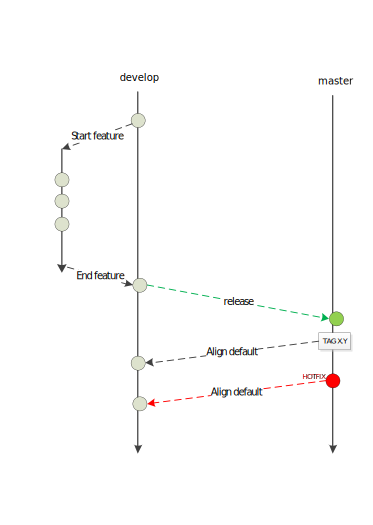
\includegraphics[width=0.5\textwidth]{img/visio-workflow-mercurial}
\end{center}
}

\fr{Rivediamo ruoli e compiti} {
\iz{
\item developer: 
    \begin{enumerate}
        \item aprono una nuova \textbf{feature branch} da default ogni volta che cominciano a sviluppare una nuova funzionalità
        \item le \textbf{feature} in realtà si aprono solo per funzionalità ``grandi'', altrimenti si lavora su default
        \item effettuano commit regolari sulla feature branch
        \item terminato lo sviluppo effettuano la merge della feature in default. Non sempre!
        \item si occupano anche degli hotfix
    \end{enumerate}

\item technical leader: 
    \begin{enumerate}
        \item supervisiona la qualità del codice prodotto
        \item è responsabile della qualità del codice che finisce sulla default branch       
    \end{enumerate}

\item release manager:
    \begin{enumerate}
        \item effettua i rilasci, quindi...
        \item quando una nuova versione è pronta per il rilascio, effettua il merge della default in stable 
        \item effettua il tagging della release
    \end{enumerate}
}
}

\fr{Init del repo} {
\sizedcode{\tiny}{code/init.txt}
}

\fr{Apertura di una feature} {
\sizedcode{\tiny}{code/open-feature.txt}
}

\fr{Fare una release} {
\sizedcode{\tiny}{code/do-release.txt}
}

\fr{Hotfix} {
\sizedcode{\tiny}{code/hotfix.txt}
}

\fr{Per approfondimenti...} {

}
\end{document}

